\subsection{Lid-Driven Cavity}~\label{secLDC}

The Lid-Driven Cavity is a canonical benchmark for incompressible viscous flow solvers~\cite{Ghia1982}. The problem consists of a square domain $\Omega = [0, L] \times [0, L]$ with $L = 1$ (dimensionless) in which the top wall moves at constant velocity $U = 1$ in the $x$-direction while all other walls are stationary. No thermal effects are present; the flow is driven entirely by the shear stress imparted by the moving lid, which sets up a large primary recirculation vortex that fills the cavity.

The flow regime is characterised by the Reynolds number:

\begin{equation}\label{eqReynolds}
    Re = \frac{\rho\,U\,L}{\mu}
\end{equation}

As $Re$ increases, inertial effects shift the primary vortex centre downstream and secondary counter-rotating vortices develop in the cavity corners. The reference case is $Re = 1000$, which lies in the inertia-dominated regime and presents sufficiently high local Peclet numbers to expose differences between convective schemes. The reference solution is provided by Ghia et al.~\cite{Ghia1982}, who tabulate the $u$-velocity along the vertical mid-plane $x = 0.5$ and the $v$-velocity along the horizontal mid-plane $y = 0.5$.


\subsubsection{Model Implementation}

The Lid-Driven Cavity uses the full NS solver described above with the energy equation (Eq.~\eqref{eqNSEnergy}) deactivated, since the problem is isothermal. The domain is a single uniform material with $\rho = 1$ and viscosity $\mu = 1/Re$, so that $L = U = 1$ satisfies Eq.~\eqref{eqReynolds} by construction.

Boundary conditions follow Section~\ref{secNSBC}: no-slip on the west, east, and south walls; moving lid ($u = 1,\ v = 0$) on the north wall. Initial conditions are $\mathbf{v}^0 = \mathbf{0}$ and $P^0 = 0$ throughout the domain. The simulation advances in time until a steady-state criterion is met, defined as the relative change in the $L_2$ norm of the velocity field falling below the specified temporal tolerance $\varepsilon_\text{temporal}$:

\begin{equation}\label{eqLDCSteadyState}
    \frac{\|\mathbf{v}^{n+1} - \mathbf{v}^n\|_2}{\|\mathbf{v}^n\|_2} < \varepsilon_\text{temporal}
\end{equation}

The velocity field output at steady state is extracted via Field probes, which record the full 2D distribution of $u$ and $v$ at each saved time step.


\subsubsection{Numerical Parameter Study}

Two independent parameter studies are carried out before the validation runs. The first establishes the minimum uniform mesh resolution that captures the primary vortex structure. The second assesses whether a non-uniform mesh, clustered toward the walls using the hyperbolic tangent distribution controlled by the $\delta$ parameter, provides accuracy gains over a uniform mesh at the same node count.

\paragraph{Mesh Refinement}
Four uniform meshes are swept using the CDS scheme at $Re = 1000$. The minimum $u$-velocity along the vertical centreline $x = 0.5$, denoted $u_{\min}$, is tracked as a scalar convergence metric and compared against the Ghia reference value. The tested values are summarised in Table~\ref{tabLDCNumerical}.

\begin{table}[ht]
    \centering
    \begin{tabular}{|c|c|}
        \hline
        Parameter & Values \\
        \hline
        $N$ & 16,\ 32,\ \textbf{64},\ 128 \\
        \hline
    \end{tabular}
    \caption{Mesh sizes tested in the spatial refinement study for the Lid-Driven Cavity ($Re = 1000$, CDS). Bold value indicates the resolution selected for subsequent studies.}
    \label{tabLDCNumerical}
\end{table}

The convergence of $u_{\min}$ with $N$ and the corresponding evolution of the centreline profiles are shown in Fig.~\ref{figLDCRefinement}.

\begin{figure}[ht]
    \centering
    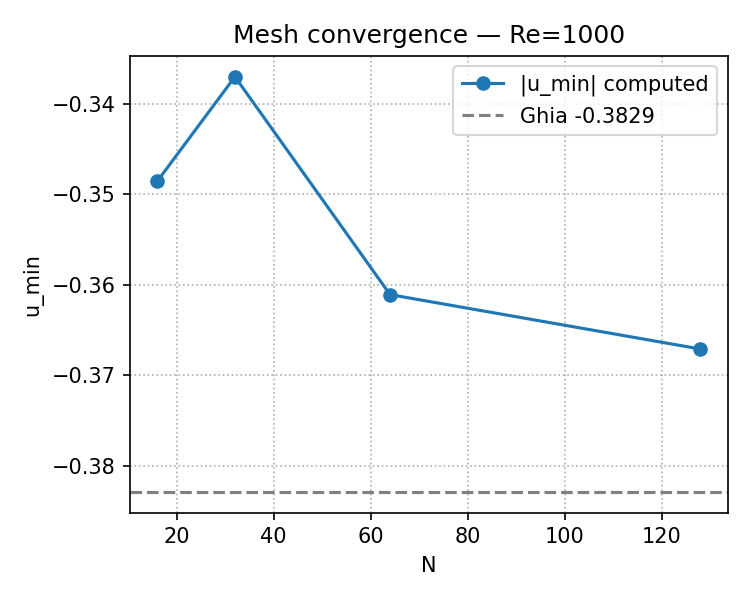
\includegraphics[width=0.45\linewidth]{Chapter3/Media/LDCRefineConvergence.png}
    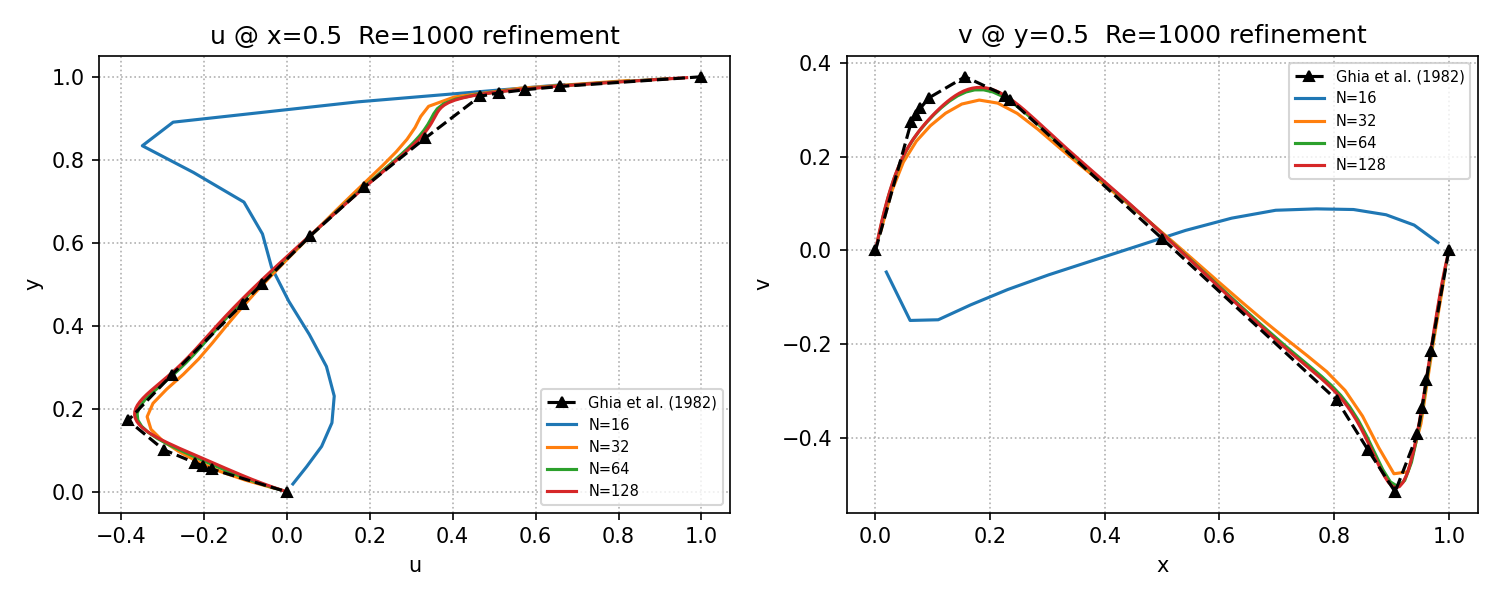
\includegraphics[width=\linewidth]{Chapter3/Media/LDCRefineProfiles.png}
    \caption{Mesh refinement study for the Lid-Driven Cavity ($Re = 1000$, CDS). Top: minimum $u$-velocity $u_{\min}$ at $x = 0.5$ as a function of $N$, compared against the Ghia reference. Bottom: centreline $u$ (left) and $v$ (right) profiles at each mesh level.}
    \label{figLDCRefinement}
\end{figure}

\paragraph{Non-uniform Mesh Study}
With the uniform resolution established, the effect of wall clustering is assessed. The hyperbolic tangent mesh distribution concentrates nodes near the walls with a stretching controlled by the $\delta$ parameter: larger $\delta$ produces stronger clustering. Four values of $\delta$ are tested at $N = 64$ and $Re = 1000$; the sensitivity of $u_{\min}$ and the corresponding centreline profiles are shown in Fig.~\ref{figLDCDelta}.

\begin{figure}[ht]
    \centering
    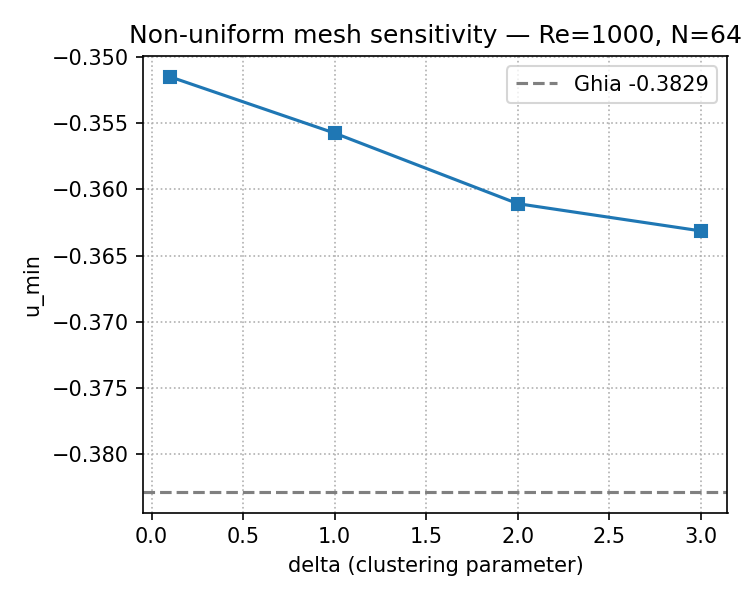
\includegraphics[width=0.45\linewidth]{Chapter3/Media/LDCDeltaSensitivity.png}
    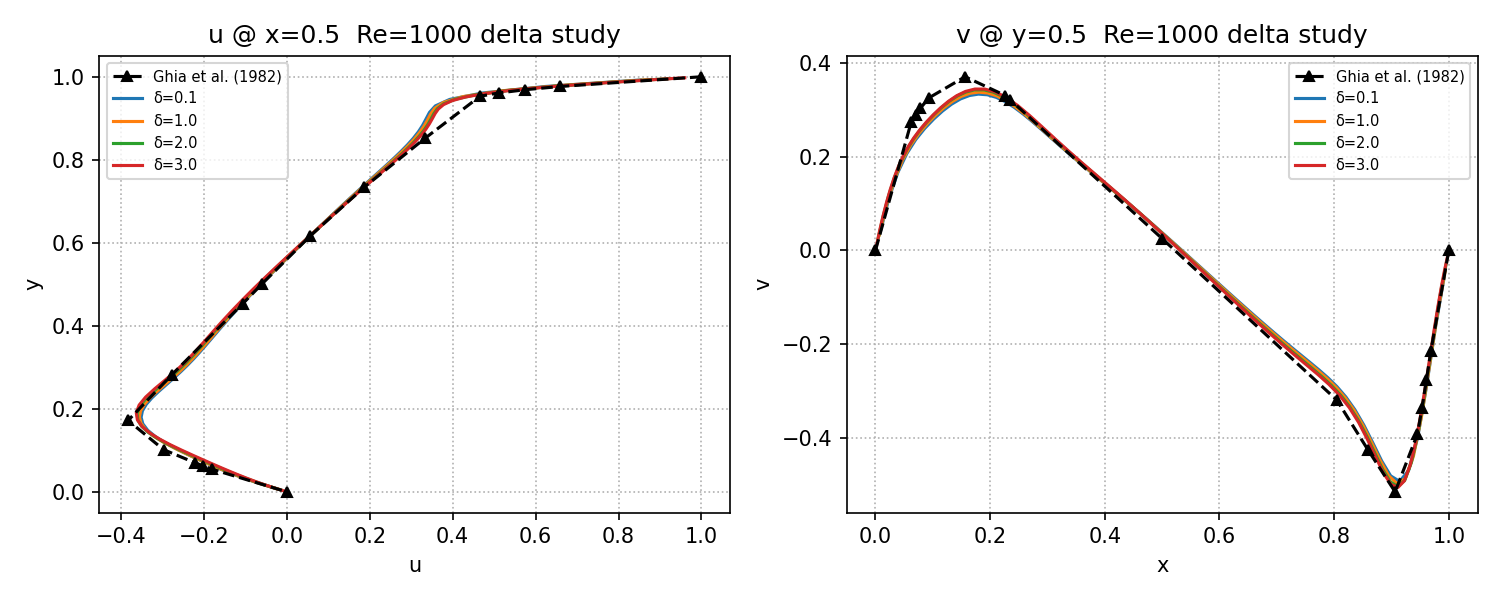
\includegraphics[width=\linewidth]{Chapter3/Media/LDCDeltaProfiles.png}
    \caption{Non-uniform mesh sensitivity for the Lid-Driven Cavity ($Re = 1000$, $N = 64$, CDS). Top: minimum $u$-velocity $u_{\min}$ as a function of the clustering parameter $\delta$, compared against the Ghia reference. Bottom: centreline $u$ (left) and $v$ (right) profiles for each $\delta$ value.}
    \label{figLDCDelta}
\end{figure}


\subsubsection{Model Validation}

The model is validated at $Re = 1000$ by comparing the steady-state centreline velocity profiles against the reference data of Ghia et al.~\cite{Ghia1982} for two convective schemes: CDS and Hybrid. At this Reynolds number the local Peclet numbers in the core of the cavity are high enough that the choice of scheme has a visible impact on the predicted profile shape, making this a meaningful scheme comparison. The $u$-velocity along the vertical centreline $x = 0.5$ and the $v$-velocity along the horizontal centreline $y = 0.5$ are the standard metrics for this benchmark. The results are presented in Fig.~\ref{figNSVelComp}.

\begin{figure}[ht]
    \centering
    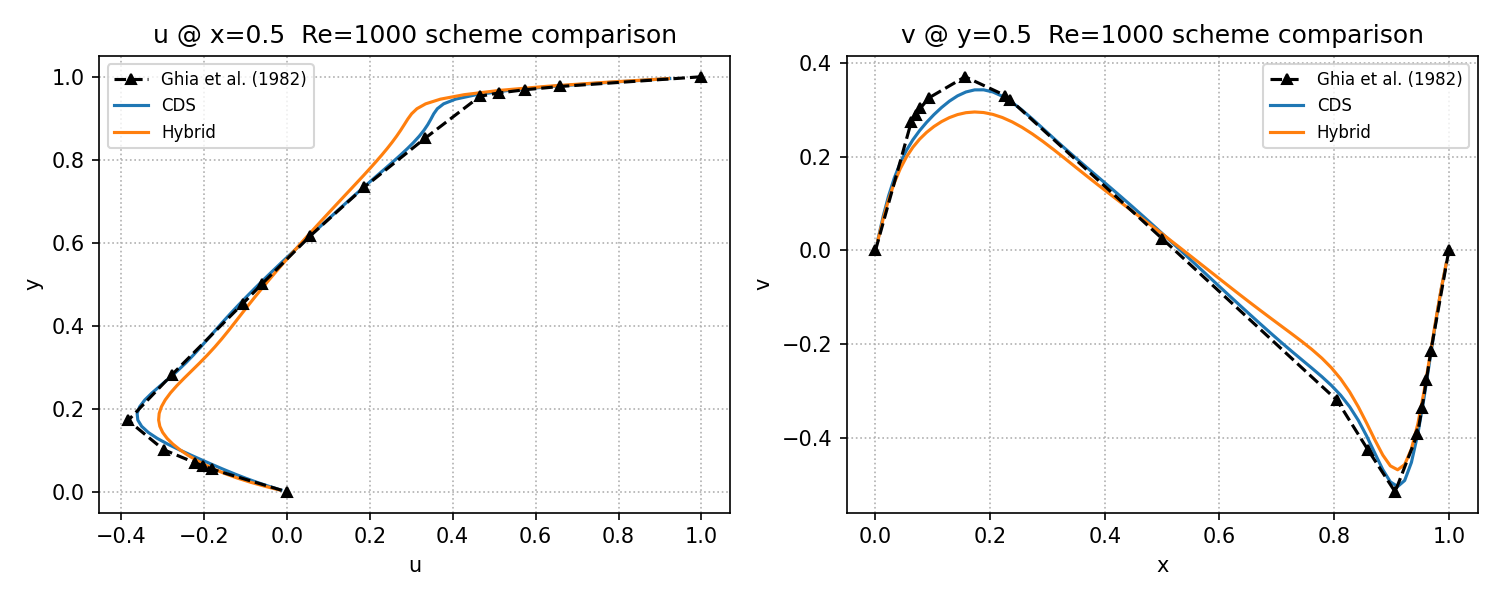
\includegraphics[width=\linewidth]{Chapter3/Media/LDCSchemeComparison.png}
    \caption{Comparison of computed centreline velocity profiles (CDS and Hybrid) against reference values of Ghia et al.~\cite{Ghia1982} at $Re = 1000$. Left: $u$-velocity along $x = 0.5$. Right: $v$-velocity along $y = 0.5$.}
    \label{figNSVelComp}
\end{figure}

The steady-state velocity magnitude colormaps and vector maps are shown in Figs.~\ref{figNSVelMag} and~\ref{figNSVelVec}, providing a qualitative picture of the vortex structure for each scheme.

\begin{figure}[ht]
    \centering
    \begin{tabular}{cc}
        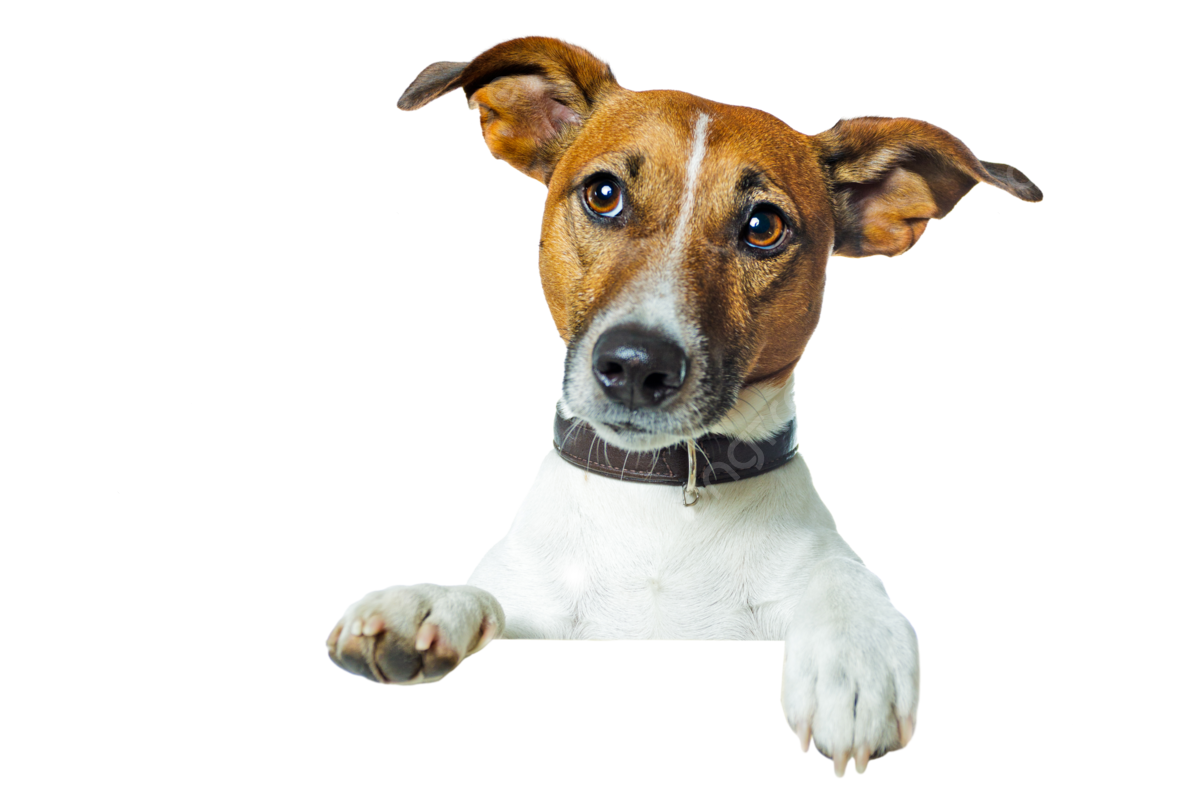
\includegraphics[width=0.45\linewidth]{Chapter3/Media/PLACEHOLDER.png} & 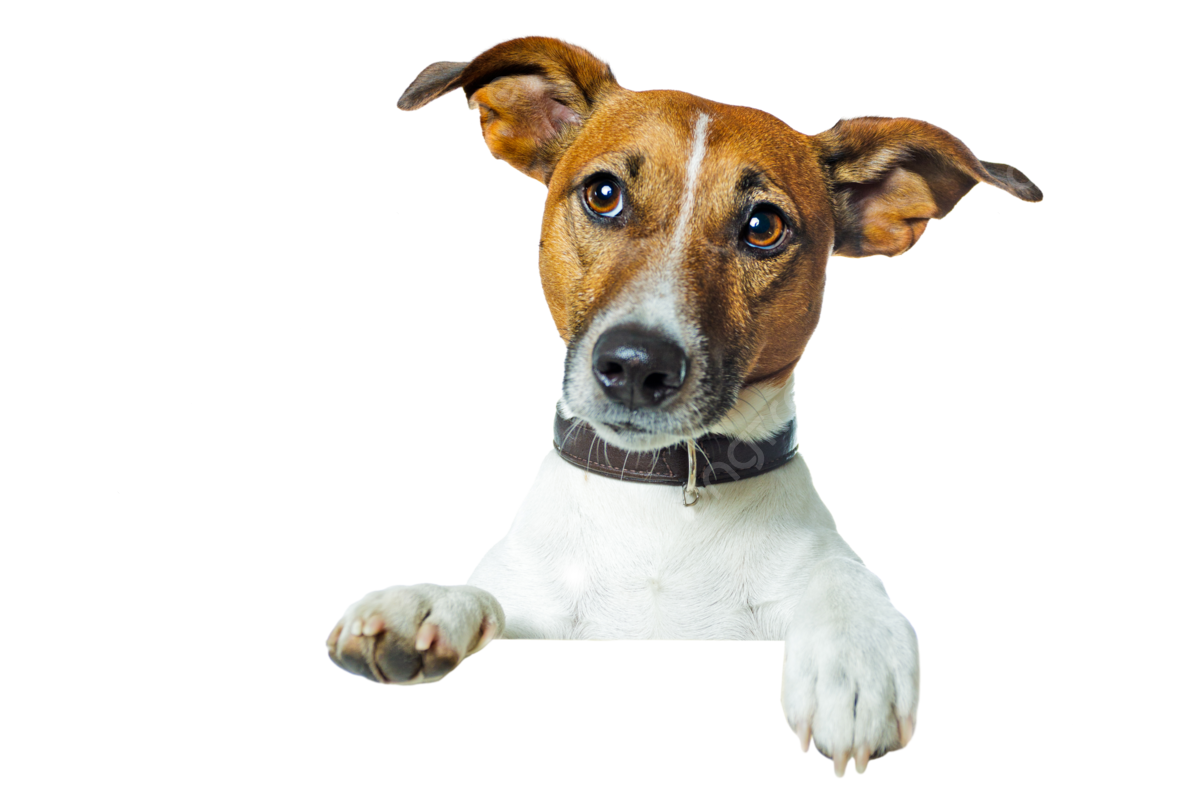
\includegraphics[width=0.45\linewidth]{Chapter3/Media/PLACEHOLDER.png} \\
        \scriptsize{\textit{CDS: $Re = 1000$}} & \scriptsize{\textit{Hybrid: $Re = 1000$}} \\
    \end{tabular}
    \caption{Steady-state velocity magnitude distribution for the Lid-Driven Cavity at $Re = 1000$, comparing CDS (left) and Hybrid (right).}
    \label{figNSVelMag}
\end{figure}

\begin{figure}[ht]
    \centering
    \begin{tabular}{cc}
        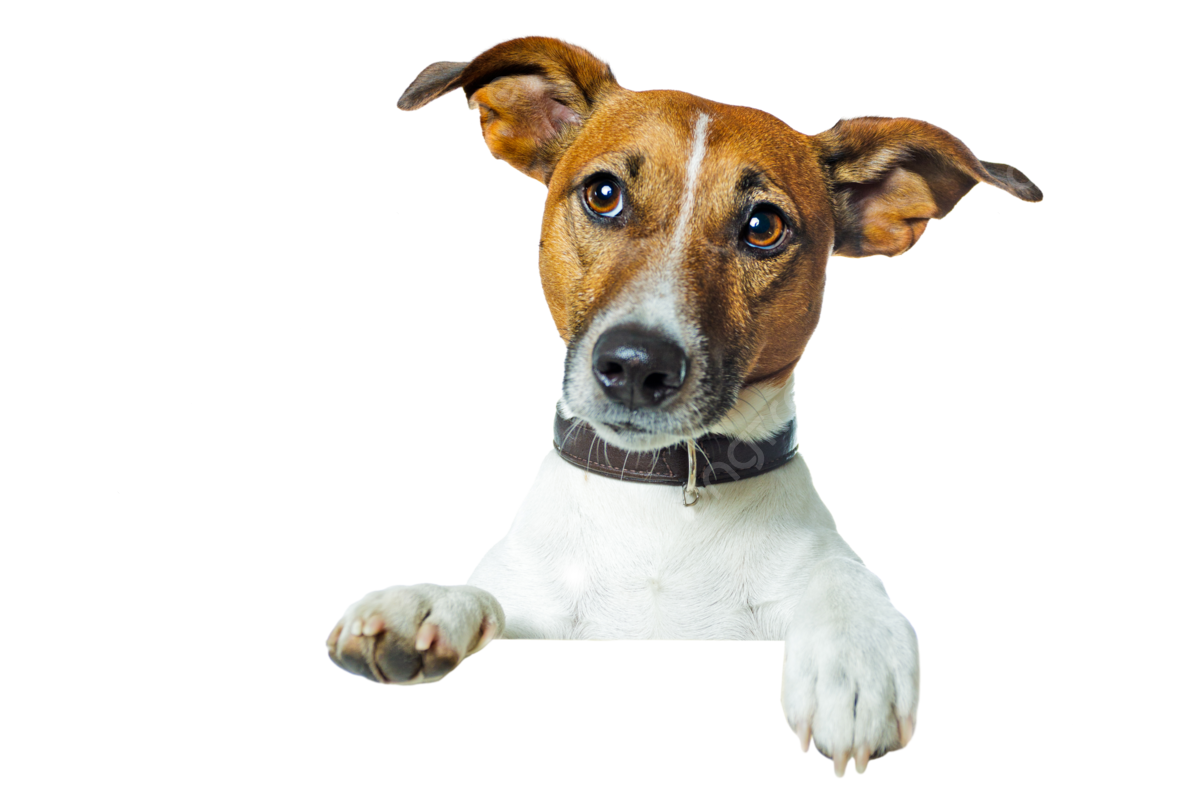
\includegraphics[width=0.45\linewidth]{Chapter3/Media/PLACEHOLDER.png} & 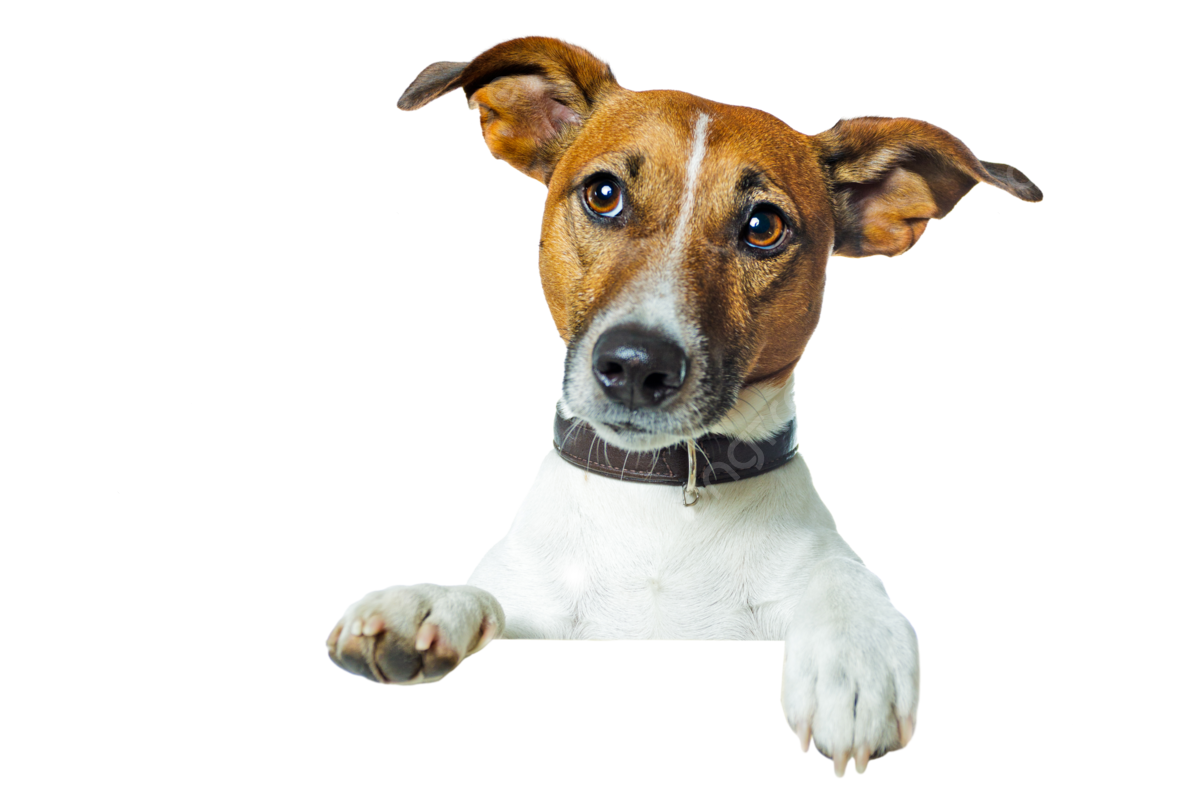
\includegraphics[width=0.45\linewidth]{Chapter3/Media/PLACEHOLDER.png} \\
        \scriptsize{\textit{CDS: $Re = 1000$}} & \scriptsize{\textit{Hybrid: $Re = 1000$}} \\
    \end{tabular}
    \caption{Steady-state velocity vector maps for the Lid-Driven Cavity at $Re = 1000$, comparing CDS (left) and Hybrid (right).}
    \label{figNSVelVec}
\end{figure}
